
\graphicspath{{./fig_2Dpoiseuille/}}

\subsection{二次元Poiseuille流}

%
\subsubsection{目的}
本例題は,二次元のPoiseuille流をPPLT2D組み込み例題クラスを用いて解析することにより,CBCソルバーの動作検証と予測精度を明らかにする.

%
\subsubsection{問題の定義と厳密解}
いま,2枚の平行平板間の定常な流れを考える.2枚の板を固定して,圧力勾配によって流体を押し流すときの流れを二次元のPoiseuilleの流れ(two-dimensional Poiseuille flow)という\cite{imai:73}.\\

平行平板の間隔を$h$とし,静止壁面上に$x$軸を選べば,運動方程式は,\ref{subsection:2Dcouette}圧力勾配のある二次元Couette流の場合と同じく,
\begin{equation}
\frac{dp}{dx}=\mu\frac{d^2u}{dy^2}
\end{equation}
となり,境界条件は,
\begin{equation}
\begin{array}{lll}
y=0 & : & u=0 \\
y=h & : & u=0
\end{array}
\end{equation}
解は次のようになる.
\begin{equation}
u(y)=-\frac{h^2}{2\mu}\frac{dp}{dx}\frac{y}{h}
\left(1-\frac{y}{h}\right)
\mbox{  }0\leq y\leq h
\end{equation}

平板間の中心線$y=h/2$に関して対称な放物線形の速度分布を持つ(\textbf{図\ref{Fig.poiseuilleG}}).
図中の$P$は無次元圧力勾配

\begin{equation}
P = \frac{h^2}{2\mu}\frac{1}{U}\left(-\frac{dp}{dx}\right)
\end{equation}
である.

\begin{figure}[htbp]
\centering
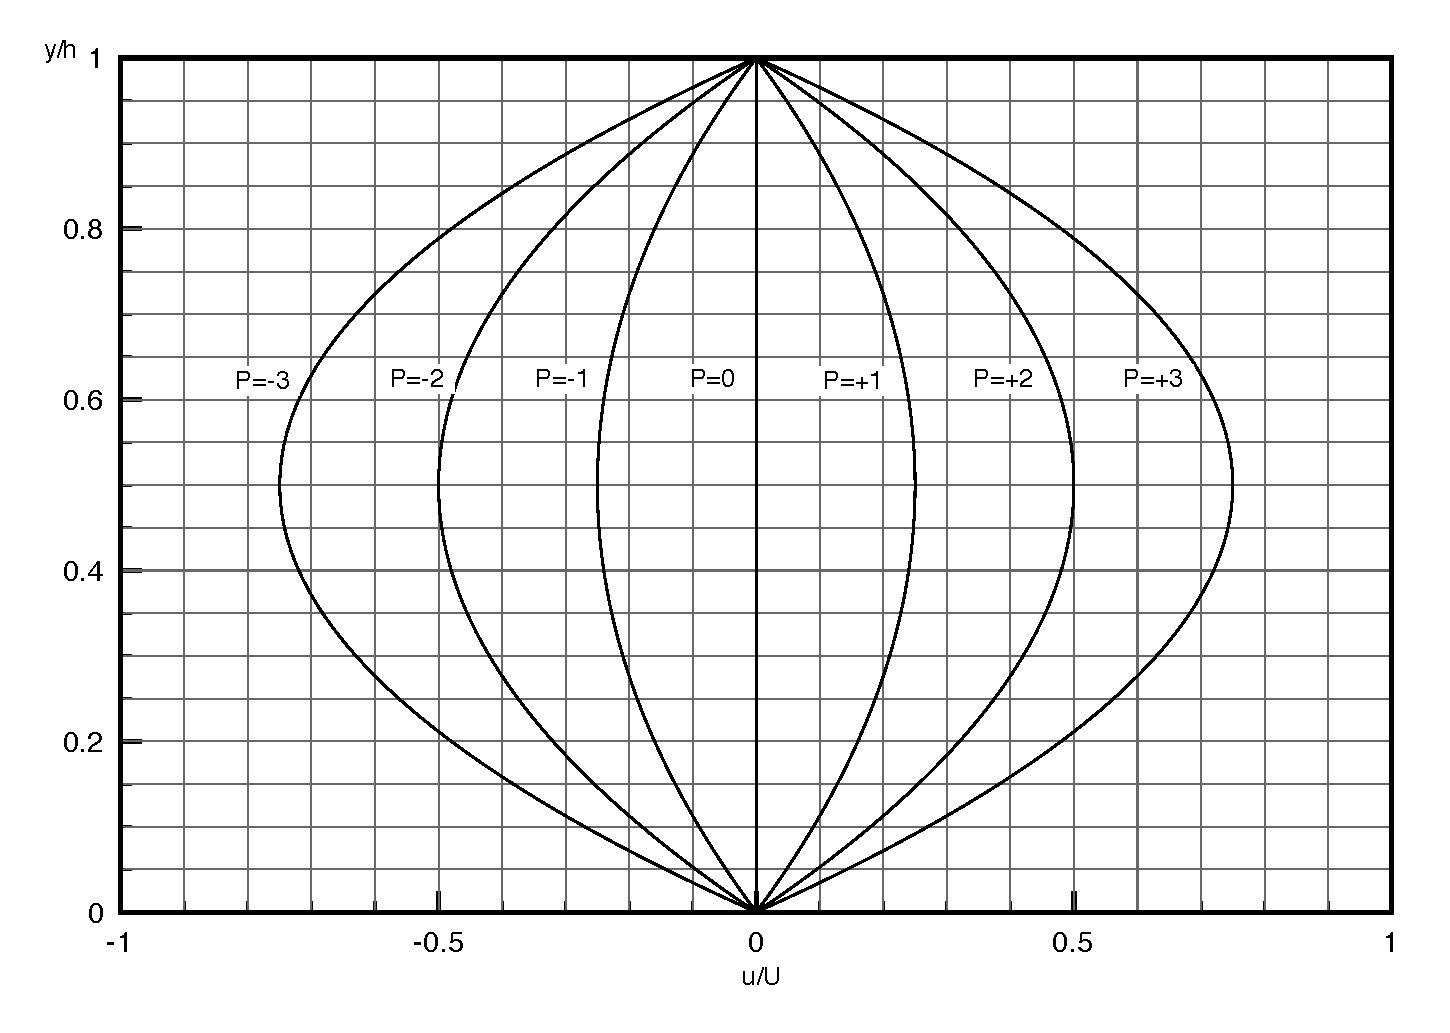
\includegraphics[width=12cm]{2DpoiseuilleG.eps}
\caption{二次元のPoiseuille流の圧力勾配に対する流速分布}
\label{Fig.poiseuilleG}
\end{figure}

\subsubsection{領域設定}
PPLT2Dクラスは辺長比が2:1の二次元空間を表現する.
$z$方向には3セルを設けており,\textbf{図\ref{Fig.poiseuilleP}}に示すように,単純な周期境界条件を用いて二次元を近似している.
本計算では,$100\times50\times3$のセル分割とした.

コンフィギュレーションファイルの\lq\lq Example\rq\rq タグで\lq\lq Parallel\_Plate\_2D\rq\rq を指定する.
Poiseuille流を再現するために,$x$軸方向に圧力勾配をかけた周期境界条件を設定し,$y=0$面,$y=h$面はは固定壁とみなし,$z\pm$面には単純な周期境界条件を与える.

\begin{figure}[htbp]
\centering
\includegraphics[width=12cm, bb=0 0 647 404]{model.png}
\caption{計算領域の設定}
\label{Fig.poiseuilleP}
\end{figure}

%\pagebreak
\subsubsection{計算環境}
本計算に利用した計算機環境とソフトウェアを\textbf{表\ref{tbl: 2dpoiseuille env}}に示す.

\begin{table}[htdp]
\small
\caption{計算機環境および利用ソフトウェア}
\begin{center}
\begin{tabular}{ll}\toprule
Computer & eX. COMPUTER\\
CPU & Intel Core i7-950 (4 Cores/CPU)$\times$ 2\\
Clock & 3.07 GHz\\
Memory & 12GB \\
Cache & 8 MB(each CPU)\\
%Cache(3rd) & 4MB\\ 
OS & Linux ubuntu 2.6.32-25-generic\\ \hline
MPI & OpenMPI 1.4.3\\
V-Sphere & ver. 1.8.4\\
CBC & ver. 1.3.8\\
FlowBase & ver. 2.3.8\\ \hline
Compiler & Intel Compiler Composer XE(12.0) 2011.3.174 C++/Fortran\\
Compile Option & -O3\\
\bottomrule
\end{tabular}
\end{center}
\label{tbl: 2dpoiseuille env}
\end{table}


%
\subsubsection{計算パラメータ}
計算に用いたパラメータ(\textbf{表\ref{Table.poi_param}}),流体の物性値(\textbf{表\ref{Table.poi_bussei}})などを示す.
\begin{table}[htbp]
\centering
\caption{計算に用いたパラメータ}
\label{Table.poi_param}
\begin{tabular}{llll}\toprule
$h$ &短辺の長さ &$1.0$ &[m]\\
$U$ &代表速度 & $1.0$ &[m/s]\\
$\Delta p$ &$x\pm$面間の圧力差($P=1$に相当) &$4.7052\times10^{-2}$ &[Pa]\\
$\nu $ & クーラン数 & 0.2 & \\
\bottomrule
\end{tabular}
\end{table}

\begin{table}[htbp]
\centering
\caption{計算に用いた物性値}
\label{Table.poi_bussei}
\begin{tabular}{llll}\toprule
物性 &&物性値  & [単位]\\
\midrule
$\rho$ & 密度 & 1.1763 & kg/m$^3$\\
$\mu$  & 粘性係数 & 1.1763 $\times 10^{-2}$ &[Pa $\cdot$ s]\\
\bottomrule
\end{tabular}
\end{table}

\textbf{表\ref{Table.poi_param}},\textbf{表\ref{Table.poi_bussei}}から,レイノルズ数は,Re=$\rho U h/\mu=100$となる.
レイリーの問題から,時間$t$[s]の間に壁の影響が粘性を通じて及ぶ距離$\delta$[m]は,$\delta=\sqrt{t\nu}$.$\nu$は動粘性係数[m$^2$/s].無次元にすると$t^*=\delta^{*2}\cdot Re$となり,$\delta^*=1$,Re=100より,計算時間をt=100[-]と見積もった.

\paragraph{サンプリングの指定}
値のサンプリングは,$z=h/2, x=h$上の$y=0 \sim h$の範囲を分割してサンプリングする.今回の計算では,分割数を25とした.

\paragraph{外部境界条件}コンフィギュレーションファイルの中で,外部境界条件において,圧力勾配($P=+1$)をかける周期境界条件と,単純な周期境界条件($z\pm$面)を設定する指定内容を示す.
{\small
\begin{program}
         <OuterBoundary>
            <Elem name="Basic_BCs">
                <Elem id="1" name="Wall">
                    <Param dtype="REAL" name="Normal_X" value="0.0"/>
                    <Param dtype="REAL" name="Normal_Y" value="0.0"/>
                    <Param dtype="REAL" name="Normal_Z" value="0.0"/>
                    <Param dtype="STRING" name="Specified_Type" value="Velocity"/>
                    <Param dtype="STRING" name="Profile" value="Constant"/>
                    <Param dtype="REAL" name="Specified_Value" value="0.0"/>
                </Elem>
                <Elem id="7" name="periodic">
                    <Param dtype="STRING" name="mode" value="Simple_Copy"/>
                </Elem>
                <Elem id="8" name="periodic">
                    <Param dtype="STRING" name="mode" value="Directional"/>
                    <Param dtype="STRING" name="flow_direction" value="upstream"/>
                    <Param dtype="REAL" name="pressure_difference" value="0.047052"/>
                </Elem>
                <Elem id="9" name="periodic">
                    <Param dtype="STRING" name="mode" value="Directional"/>
                    <Param dtype="STRING" name="flow_direction" value="downstream"/>
                    <Param dtype="REAL" name="pressure_difference" value="0.047052"/>
                </Elem>
            </Elem>
            <Elem name="Face_BC">
                <Elem comment="periodic_u" id="8" name="X_minus">
                    <Param id="600" name="Cell_ID"/>
                </Elem>
                <Elem comment="periodic_d" id="9" name="X_plus">
                    <Param id="600" name="Cell_ID"/>
                </Elem>
                <Elem comment="wall" id="1" name="Y_minus">
                    <Param id="600" name="Cell_ID"/>
                </Elem>
                <Elem comment="slide_wall" id="1" name="Y_plus">
                    <Param id="600" name="Cell_ID"/>
                </Elem>
                <Elem comment="periodic" id="7" name="Z_minus">
                    <Param id="600" name="Cell_ID"/>
                </Elem>
                <Elem comment="periodic" id="7" name="Z_plus">
                    <Param id="600" name="Cell_ID"/>
                </Elem>
            </Elem>
       </OuterBoundary>
\end{program}
}


%
\subsubsection{計算結果と厳密解の比較}

図\ref{Fig.poi_exact_100}に,無次元圧力勾配$P=-3, -2, -1, 0, +1, +2, +3$の場合の,厳密解(実線)およびCBCの計算結果$u/U$(マーク)の値を比較した.
CBCと厳密解の誤差は,厳密解の$10^{-4}$のオーダーに収まっており,よく一致しているといえる.


\begin{figure}[htbp]
\begin{center}
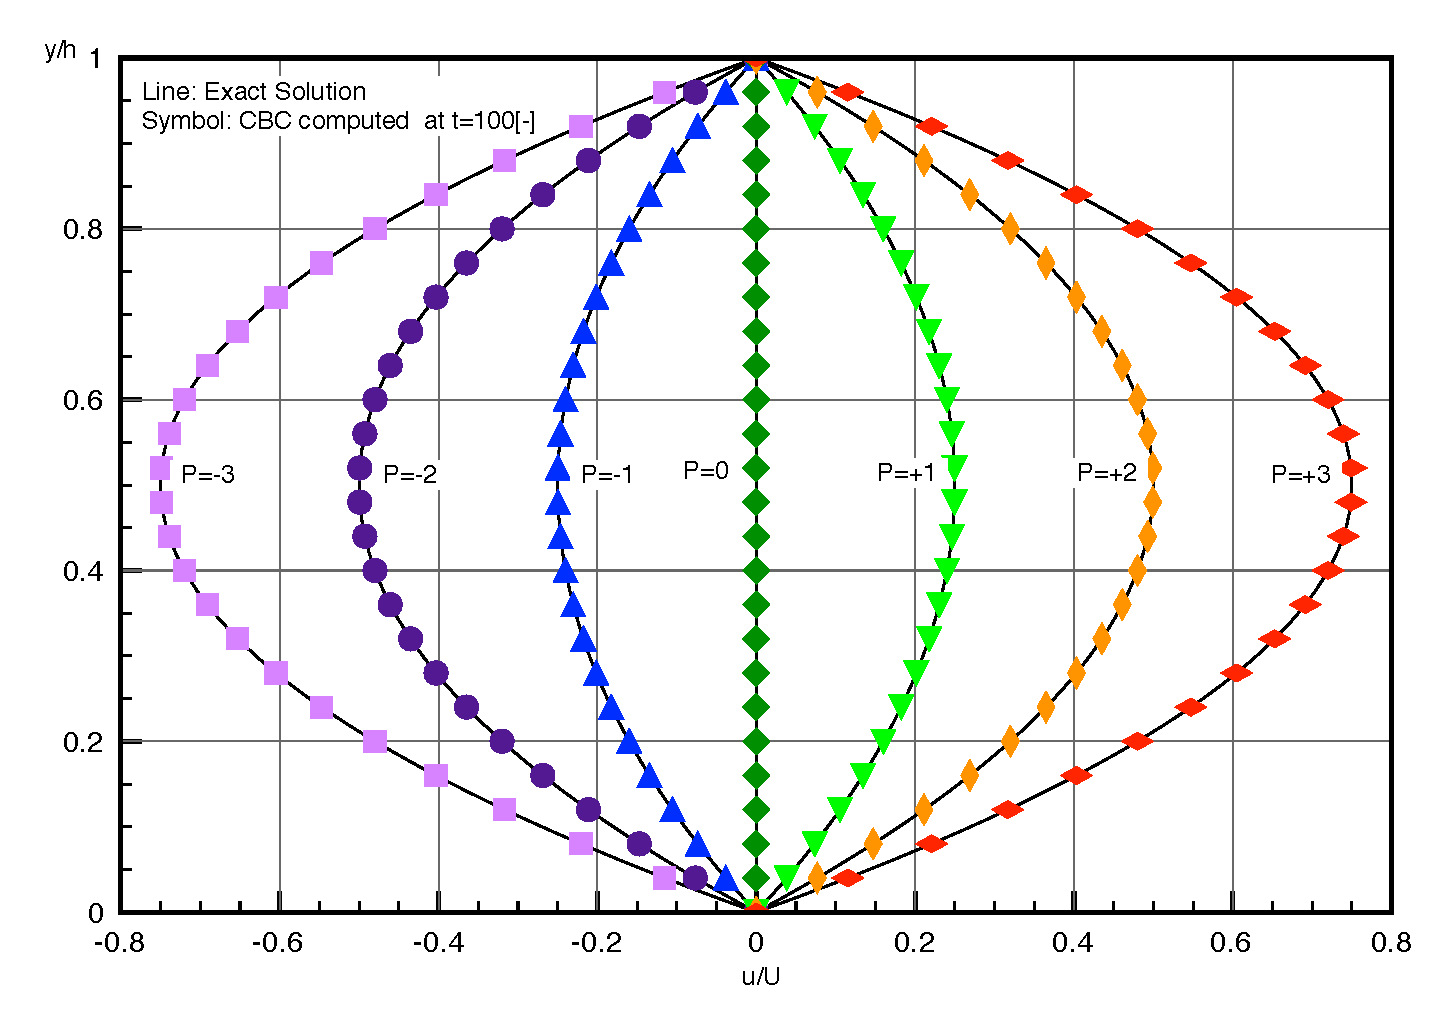
\includegraphics[width=14cm]{2Dpoiseuille_100.eps}
\end{center}
\caption{Poiseuille流の速度分布(厳密解とシミュレーションの比較)}
\label{Fig.poi_exact_100}
\end{figure}

%
\subsubsection{ファイルのメモ}
例題の提供ファイルの説明を以下に示す.\\
%\begin{quote}
%\centering
\begin{tabularx}{180mm}{lclclX}
%\hspace{12em}\= \hspace{30em}\kill
example\CID{07480}2Dpoiseuille & \CID{07530}&\CID{00718}&\CID{07530}&poiseuille.xml & 圧力勾配$*:P=-3,\,-2,\,-1,\,0,\,1,\,2,\,3$の場合のコンフィギュレーションファイル\\
&\CID{07482}&&\CID{07514}&condition.txt & conditionファイル\\
&\CID{07482}&&\CID{07514}&profiling.txt & 実行時性能測定結果ファイル\\
&\CID{07482}&&\CID{07514}&sample\_x=0.log & samplingファイル\\
&\CID{07482}&&\CID{07502}&history\_base.log& 履歴ファイル\\
%&\CID{07482}&&\CID{07502}&(error\_P=+3.plot) & $P=+3$における解析解と厳密解との誤差.図\ref{Fig.couette.error} (\url{http://plot.micw.eu/})
%\\
%&\CID{07514}&\multicolumn{3}{l}{exact.f90} & 厳密解を計算するFortranコード\\
&\CID{07502}&\multicolumn{3}{l}{2Dpoiseuille\_100.plot} &  厳密解と,$t=100[-]$における解析解の比較.\textbf{図\ref{Fig.poi_exact_100}}\\
& & &&&(\url{http://plot.micw.eu/})
\end{tabularx}
%\end{quote}
\\
\paragraph{conditionファイル内の無次元圧力勾配について}
{}~\ref{subsection:2Dcouette}圧力勾配のある二次元Couette流の同項目を参照.